\documentclass[a4paper,landscape,8pt]{extarticle}

\usepackage[a4paper,margin=0.7cm]{geometry}

\usepackage{fancyhdr}
\pagestyle{fancy}
\fancyfoot[R]{\vspace{-35pt}\Huge\thepage}

\usepackage{multicol}
\setlength\columnsep{20pt}
\setlength{\columnseprule}{0.1pt} 

\setlength\parindent{0pt}

\usepackage[ngerman]{babel} % Silbentrennung
\usepackage[utf8]{inputenc} % Umlaute
\usepackage{microtype}

\usepackage{hyperref}

\usepackage{float}
\usepackage{graphicx}

\usepackage{comment}
\usepackage{amsmath}
\usepackage{amssymb}

\usepackage{cancel}

\usepackage{color}
\usepackage{xcolor}

\usepackage{color}

\usepackage{booktabs}

\newenvironment{rcases}
  {\left.\begin{aligned}}
  {\end{aligned}\right\rbrace}
  
\usepackage{enumitem}
\setlist{noitemsep,topsep=3pt,parsep=3pt,partopsep=3pt,leftmargin=18pt}
\renewcommand\labelitemi{{\boldmath$\cdot$}}
\newcommand{\listarrow}{
\smash{\scalebox{1.5}[1.75]{\rotatebox[origin=c]{180}{$\Lsh$}}}
}
\usepackage{xifthen}
\newcommand{\emptyarg}[1][]{\ifthenelse{\isempty{#1}}{}{\ #1}}

% % % % %
% Structural
% % % % %

\newcommand{\Def}[1][]{\colorbox{defcolor}{\color{titlecolor}{\textbf{D\emptyarg[#1]}}}\kern+0.3ex}

\newcommand{\Satz}[1][]{\colorbox{satzcolor}{\color{titlecolor}{\textbf{S\emptyarg[#1]}}}\kern+0.3ex}

\newcommand{\Theo}[1][]{\colorbox{lemcolor}{\color{titlecolor}{\textbf{T\emptyarg[#1]}}}\kern+0.3ex}

\newcommand{\Korollar}[1][]{\colorbox{lemcolor}{\color{titlecolor}{\textbf{K\emptyarg[#1]}}}\kern+0.3ex}

\newcommand{\Trick}[1][]{\colorbox{trkcolor}{\color{titlecolor}{\textbf{Trick:\emptyarg[#1]}}}\kern+0.3ex}

\newcommand{\Vorgehen}[1][]{\colorbox{trkcolor}{\color{titlecolor}{\textbf{Vorgehen:\emptyarg[#1]}}}\kern+0.3ex}

\newcommand{\Bsp}[1][]{\colorbox{bspcolor}{\color{titlecolor}{\textbf{B\emptyarg[#1]}}}\kern+0.3ex}

% % % % %
% In Text
% % % % %

\newcommand{\Bem}{\textbf{Bem: }}
\newcommand{\Beweis}{\textbf{Beweis: }}
\newcommand{\Achtung}{\textbf{Achtung: }}
\newcommand{\Wichtig}{\textbf{Wichtig: }}

% % % % %
% Colors
% % % % %

\definecolor{defcolor}{rgb}{0.5, 1, 0.5}
\definecolor{satzcolor}{rgb}{0.5, 0.95, 1}
\definecolor{lemcolor}{rgb}{1, 0.75, 0.75}
%\definecolor{trkcolor}{rgb}{1, 0.7, 0}
\definecolor{trkcolor}{rgb}{0.7, 0.95, 1}
\definecolor{bspcolor}{rgb}{1, 0.95, 0.43}
\definecolor{titlecolor}{rgb}{0,0,0}

% % % % %
% Math
% % % % %

\DeclareMathOperator{\arcsinh}{arcsinh}
\DeclareMathOperator{\arccosh}{arccosh}
\DeclareMathOperator{\arctanh}{arctanh}
\DeclareMathOperator{\arc}{arc}

\renewcommand\div{\operatorname{div}}
\DeclareMathOperator{\rot}{rot}
\newcommand{\laplace}{\Delta}

\DeclareMathOperator{\cis}{cis}

\DeclareMathOperator{\grad}{grad}
\DeclareMathOperator{\Hess}{Hess}

\newcommand{\N}{\mathbb{N}}
\newcommand{\Z}{\mathbb{Z}}
\newcommand{\Q}{\mathbb{Q}}
\newcommand{\R}{\mathbb{R}}
\newcommand{\C}{\mathbb{C}}


\renewcommand\Re{\operatorname{Re}}
\renewcommand\Im{\operatorname{Im}}

\newcommand{\abs}[1]{\left\lvert #1 \right\rvert}
\newcommand{\norm}[1]{\left\lVert #1 \right\rVert}
\newcommand{\scprod}[1]{\left\langle #1 \right\rangle}
\newcommand{\ceil}[1]{\left\lceil #1 \right\rceil}
\newcommand{\floor}[1]{\left\lfloor #1 \right\rfloor}

\newcommand{\diag}{\operatorname{diag}}

\newcommand{\hl}[1]{\colorbox{black!7}{$#1$}}

\newcommand{\notimplies}{\;\not\!\!\!\implies}

% % % % %
% Layout
% % % % %

\newcommand{\setsep}{\ \vert \ }

\newcommand{\todo}{\textcolor{red}{TODO }}

\newcommand{\sep}{\vspace{5pt}\noindent\hrule\vspace{5pt}}


\newcommand{\veryshortarrow}[1][3pt]{\mathrel{%
   \hbox{\rule[\dimexpr\fontdimen22\textfont2-.2pt\relax]{#1}{.4pt}}%
   \mkern-4mu\hbox{\usefont{U}{lasy}{m}{n}\symbol{41}}}}
% TODO remove command
\renewcommand*{\newpage}{ \ }
%\renewcommand*{\part}{\ }
% package to define custom environments
\usepackage{environ}
% boolean variable to show contents
\newif\ifshowwarmup
%\showwarmuptrue % set it to true
\showwarmupfalse % set it to false
% definition of custom environment
\NewEnviron{warmup}{\ifshowwarmup \BODY \fi}
% shorthand for custom environment
%\def\WU#1\UW{\begin{warmup}#1\end{warmup}}
% Ultra shortening of Document
%
% http://www.terminally-incoherent.com/blog/
%2007/09/19/latex-squeezing-the-vertical-white-space/
%\setlength{\parskip}{0pt}
%\setlength{\parsep}{0pt}
%\setlength{\headsep}{0pt}
\setlength{\topskip}{0pt}
%\setlength{\topmargin}{0pt}
%\setlength{\topsep}{0pt}
%\setlength{\partopsep}{0pt}
%\linespread{0.7}
\usepackage[compact]{titlesec}
\titlespacing{\section}{0pt}{*0}{*0}
\titlespacing{\subsection}{0pt}{*0}{*0}
\titlespacing{\subsubsection}{0pt}{*0}{*0}
%\usepackage{savetrees} %(alternative)
\pagenumbering{gobble}
% Use custom numbering
%\setcounter{secnumdepth}{0}
\usepackage{centernot}
\begin{document}
\setlength{\belowdisplayskip}{4pt} \setlength{\belowdisplayshortskip}{4pt}
\setlength{\abovedisplayskip}{4pt} \setlength{\abovedisplayshortskip}{4pt}
% allow page break in align* environment
\allowdisplaybreaks
\begin{multicols*}{4} % change to 3 if you want only 3 columns
\raggedcolumns
\graphicspath{ {./img/} }
\section*{Grundlagen}
\Def[1.1Sigma-Algebra ]
\begin{itemize}
    \item \(\omega \in \mathcal{F}\)
    \item  \(A \in \mathcal{F} \implies A^c \in \mathcal{F}\)
    \item \(A_1, A_2, \dots \in \mathcal{F} \implies \bigcup_{i=1}^{\infty} A_i \in \mathcal{F} \)
\end{itemize}
\Def[1.2 Wahrscheinlichkeitsmass ]
\begin{itemize}
    \item \( \mathcal{P}[\omega] = 1\)
    \item \(\sigma-\text{Additivität} \ \mathcal{P}[A] = \sum_{i=1}^{\infty} \mathcal{P}[A_i]\) \newline if \( A = \bigcup_{i=1}^{\infty} A_i \) (disjunkte Vereinigung)
\end{itemize}
\Def[1.3 Wahrscheinlichkeitsraum ] \\
Sei \( \omega \) ein Grundraum, \(\mathcal{F}\) eine \(\sigma\) -Algebra und \(\mathcal{P}\) ein Wahrscheinlichkeitsmass. Wir nennen das Tripel\( (\omega, \mathcal{F}, \mathcal{P})\)  Wahrscheinlichkeitsraum.
\Def[1.5 Laplace Modell] \\
\begin{itemize}
    \item \(\mathcal{F} = \mathcal{P}(\omega)\)
    \item \(\mathbb{P} : \rightarrow \left[0,1\right]\) ist definiert durch \[ \forall A \in \mathcal{F} \ \mathbb{P}[A] = \frac{\abs{A}}{\abs{\omega}}\]
\end{itemize}
\Satz[1.6]
Für eine Sigma-Algebra \(\mathcal{F} \ \text{auf} \ \omega\) gilt:
\begin{itemize}
    \item \(\emptyset \in \mathcal{F}\)
    \item \(A_1, A_2, \dots \in \mathcal{F} \implies \bigcap_{i=1}^{\infty} A_i \in \mathcal{F}\)
    \item \(A,B \in \mathcal{F} \implies A \cup B \in \mathcal{F}\)
    \item \(A,B \in \mathcal{F} \implies A \cap B \in \mathcal{F}\)
\end{itemize}
\Satz[1.7]
\begin{itemize}
    \item \( \mathbb{P}[\emptyset] = 0\)
    \item \(A_1, \dots A_k\) paarweise disjunkte Ereignisse, \[\mathbb{P}[A_1 \cup \dots \cup A_k] = \mathbb{P}[A_1] + \dots \mathbb{P}[A_k]\]
    \item \( \mathbb{P}[A^c] = 1 - \mathbb{P}[A]\)
    \item \(\mathbb{P}[A \cup B ] = \mathbb{P}[A] - \mathbb{P}[B] - \mathbb{P}[A \cap B]\)
\end{itemize}
\Satz[1.8] Seien \(A,B \in \mathcal{F}\) dann gilt \[ A \subset B \implies \mathbb{P}[A] \leq \mathbb{P}[B]\]
\Satz[1.9] Sei \( A_1, A_2, \dots \) eine Folge von nicht notwendigerweise disjunkten Ereignissen, dann gilt: \[ \mathbb{P}[\bigcup_{i=1}^{\infty} A_i \leq \sum_{i=1}^{\infty} \mathbb{P}[A_i]]\]
\Def[1.13 Bedingte Wahrscheinlichkeit] \newline
Sei \((\omega, \mathcal{F}, \mathbb{P})\) ein Wahrscheinlichkeitsraum. Seien A, B zwei Ereignisse mit \( \mathbb{P}[B] > 0\) \[\mathbb{P}[A|B] = \frac{\mathbb{P}\left[A \cap B\right]}{\mathbb{P}\left[B\right]}\]
\Satz[1.16 Gesetz der totalen Wahrscheinlichkeit] \newline
Sei  \( B_1, \dots , B_n\) eine Partition des Grundraumes \( \omega \), so dass \( \mathbb{P}[B_i] > 0 \) für jedes \( 1 \leq i \leq n\) gilt. Dann gilt: \[\forall A \in  \mathcal{F} \ \mathbb{P}[A] = \sum_{i=1}^{n} \mathbb{P} \left[A | B_i \right] \mathbb{P}[B_i]\]
\Satz[1.17 Satz von Bayes] \newline
Sei \( B_1 \dots B_n \in \mathcal{F }\) eine Partition von \( \omega\) sodass, \( \mathbb{P}[B_i] > 0 \) für jedes i gilt. Für jedes Ereignis A mit \( \mathbb{P}[A] > 0 \) gilt  \[ \forall i = 1, \dots n \ \mathbb{P}\left[ B_i | A \right] = \frac{\mathbb{P}[A | B_i] \mathbb{P}[B_i]}{\sum_{j=1}^{n} \mathbb{P}[A | B_j] \mathbb{P}[B_j] }\]
\Def[1.18 Unabhängigkeit] \newline
Sei \( (\omega, \mathcal{F}, \mathbb{P})\) ein Wahrscheinlichkeitsraum. Zwei Ereignisse A und B heissen unabhängig falls \[ \mathbb{P} \left[A \cap B \right] = \mathbb{P}\left[A\right] \mathbb{P} \left[B\right]\]
\Satz[1.20] \newline
Seien A,B \( \in \mathcal{F}\) zwei Ereignisse mit \( \mathbb{P}[A], \mathbb{P}[B] > 0 \). Dann sind folgende Aussagen äquivalent:
\begin{enumerate}
    \item \( \mathbb{P}[A \cap B] = \mathbb{P}[A] \mathbb{P}[B]\)
    \item \( \mathbb{P}[A | B] = \mathbb{P}[A]\)
    \item \( \mathbb{P}[B | A] = \mathbb{P}[B]\)
\end{enumerate}
\Def[1.21]  \newline
Sei I eine beliebige Indexmenge. Eine Familie von Ereignissen \( (A_i)_{i \in I}\) heisst unabhängig falls \[ \forall J \subset I \text{endlich} \quad \mathbb{P}[\bigcap_{j \in J}A_j] = \prod_{j \in J} \mathbb{P}[A_j]\]
\Bem \newline
Drei Ereignisse A,B und C sind unabhängig falls alle 4 folgenden Gleichungen erfüllt sind
\begin{enumerate}
    \item \( \mathbb{P}[A \cap B ] = \mathbb{P}[A] \mathbb{P}[B]\)
    \item \( \mathbb{P}[A \cap C ] = \mathbb{P}[A] \mathbb{P}[C]\)
    \item \( \mathbb{P}[B \cap C ] = \mathbb{P}[B] \mathbb{P}[C]\)
    \item \( \mathbb{P}[A \cap B \cap C  ] = \mathbb{P}[A] \mathbb{P}[B] \mathbb{P}[C]\)
\end{enumerate}
\sep
\section{Zufallsvariablen und Verteilungsfunktionen}
\subsection{Abstrakte Definition }
\Def[2.1 Zufallsvariable] \newline
Sei \( (\omega, \mathcal{F}, \mathbb{P})\) ein Wahrscheinlichkeitsraum. Eine Zufallsvariable ist eine Abbildung \( X : \omega \rightarrow \mathbb{R} \) so dass, für alle \( a \in \mathbb{R}\) gilt \[ \{ w \in \omega : X(w) \leq a \} \in \mathcal{F}\]
\Bem  \newline
Für Ereignisse im Bezug auf Z:V
\begin{itemize}
    \item \( \{X \leq a \} = \{ w \in \omega : X(w) \leq a\}\)
    \item \( \{ a < X \leq b \} = \{ w \in \omega : a < X(w) < b\}\)
    \item \( \{ X \in \mathbb{Z}\} = \{ w \in \omega : X(w) \in \mathbb{Z}\}\)
\end{itemize}
\[ \mathbb{P}[X \leq a] = \mathbb{P}[\{X \leq a\}] = \mathbb{P}[\{w \in \omega : X(w) \leq a\}]\]
\subsection{Verteilungsfunktion}
\Def[2.2 Verteilungsfunktion] \newline
Sei X eine Zufallsvariable auf einem W-Raum \( (\omega, \mathcal{F}, \mathbb{P})\). Die Verteilungsfunktion von X ist eine Funtkion \(F_X : \mathbb{R} \rightarrow [0,1]\), definiert durch \[ \forall a \in \mathbb{R} \ F_X(a) = \mathbb{P}[X \leq a]\]
\Satz[2.3 Einfache Identität] \newline
Seien \(a < b\) zwei reelle Zahlen. Dann gilt \[ \mathbb{P}[a < X \leq b ] = F(b) - F(a)\]
\Theo[2.4 Eigenschaften der Verteilungsfunktion] \newline
Sei X eine Z.V aif einem Wahrscheinlichkeitsraum. Die Verteilungsfunktion \( F = F_X : \R \rightarrow [0,1]\) von X erfüllt folgende Eigenschaften
\begin{itemize}
    \item F ist monoton wachsend
    \item F ist rechtsstetig
    \item \( \lim_{a \rightarrow -\infty} F(a) = 0 \) und \( \lim_{a \rightarrow \infty} F(a) = 1\)
\end{itemize}
\subsection{Unabhängigkeit von Zufallsvariablen}
\Def[2.5] \newline
Seien \( X_1 \dots X_n \) Zufallsvariablen auf einem W-Raum. Dann heissen \(X_1, \dots X_n \) unabhängig falls \[ \forall x_1, x_2 \dots x_n \in \R \] \[\mathbb{P}[X_1 \leq x_1 \dots X_n \leq x_n ] = \mathbb{P}[X_1 \leq x_1] \dots \mathbb{P}[X_n \leq x_n]\]
\Satz[2.7 Gruppieren von Zufallsvariablen] \newline
Seien \(X_1 \dots X_n\) n unabhängige Zufallsvariablen. Seien \( 1 \leq i_1 < i_2 < \dots < i_k \leq n \) Indizes und \(\phi_1 \dots \phi_k\) Abbildungen. Dann sind  \[ Y_1 = \phi_1(X_1 \dots X_{i_1}), Y_2 = \phi_2(X_{i_{1}+1}, \dots X_{i_2}), \dots \] \[Y_k = \phi_k(X_{i_{k-1}+1} \dots X_{i_k})\] unabhängig \newline
\newline \newline
\Def[2.8] \newline
Eine Folge von Zufallsvariablen \(X_1, X_2, \dots \) heisst
\begin{itemize}
    \item unabhängig falls \(X_1, \dots X_n \) unabhängig sind, für alle \(n \in  \N\)
    \item unabhängig und identisch verteilt(uiv) falls sie unabhängig ist und die Zufallsvariablen dieselbe Verteilungsfunktion haben d.h \[ \forall i, j \ F_{X_i} = F_{X_j}\]
\end{itemize}
\subsection{Konstruktion von Zufallsvariablen}
\Def[2.9] \newline
Sei \(p \in [0,1]\). Eine Zufallsvariable X heisst Bernoulli ZUfallsvariable mit Parameter p falls \[\mathbb{P}[X=0] = 1 - p \ \text{und} \ \mathbb{P}[X=1] = p\]
Dabei schreiben wir \( X \sim Ber(p)\)
\Theo[2.10 Existenzsatz von Kolmogorov] \newline
Es existiert ein W-Raum \( (\Omega, \mathcal{F}, \mathbb{P}) \) und eine nicht endliche uiv Folge von Bernoulli Zufallsvariablen \(X_1, X_2, \dots \) auf \( (\Omega, \mathcal{F}, \mathbb{P}) \) mit Paramter \(\frac{1}{2}\)
\Def[2.11] \newline
Eine Zufallsvariable U heisst gleichverteilt auf \([0,1]\) falls ihre Verteilungsfunktion gegeben ist durch\[F_U(x) = \left.
    \begin{cases}
    0 & x < 0 \\
    x & 0 \leq x \leq 1 \\
    1 &  x > 1
\end{cases}
\right.\]
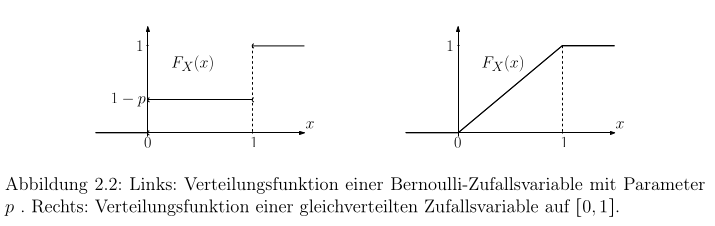
\includegraphics[scale=0.3]{abb2.2.png}
\Def[2.13 Pseudoinverse] \newline
Die Pseudoinverse von F ist eine Abbildung \(F^{-1} : (0,1) \rightarrow \R \) definiert durch \[ \forall \alpha \in (0,1) \ F^{-1} = \inf{x \in \R : F(x) \geq \alpha}\]
Nach Definition des Infimums und unter Verwendung der rechten Stetigkeit von F ergibt sich für jedes \(x \in \R \) und \( \alpha \in (0,1)\)
\[ (F^{-1}(\alpha) \leq x ) \Leftrightarrow (\alpha \leq F(x))\]
\Theo[2.14 Inversionsmethode] \newline
Sei \(F: \rightarrow [0,1]\) eine Abbildung, welche Eigenschaften 1-3 erfüllt. Sei U eine Gleichverteilte Zufallsvariable. Dann besitzt die Zufallsvariable
\[X = F^{-1}(U)\]
gerade die Verteilungsfunktion \(F_X = F\)

\sep
\section{Diskrete und stetige Variablen}
\subsection{Unstetigkeit/Stetigkeit der Verteilungsfunktion F}
\Satz[3.1 Wahrscheinlichkeit eines Punktes] \newline
Sei \( X : \omega \rightarrow \R \) eine Zufallsvariable mit Verteilungsfunktion F. Für jdedes a in \(\R\) gilt \[ \mathbb{P}[X = a] = F(a) - F(-a)\]
\subsection{Fast sichere Ereignisse}
\Def[3.2] \newline
Sei \( A \in \mathcal{F} \) ein Ereignis. Wir sagen A tritt fast sicher ein falls \[ \mathbb{P}[A] = 1\]
\subsection{Diskrete Zufallsvariablen}
\Def[3.4 Diskrete Zufallsvariable] \newline
Eine Zufallsvariable \( X : \omega \rightarrow \R \) hiest diskret falls eine endliche oder abzählbare Menge \( W \subset \R\) existiert, sodass \[ \mathbb{P}[X \in W ] = 1\]
\Bem[3.5] Wenn der Grundraum \( \omega\) endlich oder abzähbar ist, dann ist jede Zufallsvariable \( X : \omega \rightarrow \R\) diskret. \newline
\Def[3.6 Verteilung von X] \newline
Sei X eine diskrete Zufallsvariable mit Werten in einer endlichen oder abzähbaren Menge \( W \subset \R\). Die Zahlenfolge \((p(x))_{x \in W}\) definiert durch \[ \forall x \in W \ p(x) := \mathbb{P}[X = x]\] heisst Verteilung von X \newline
\Satz[3.7] Die Verteilung \((p(x))_{x \in W}\) einer diskreten Zufallsvariable erfüllt \[ \sum_{x \in W} p(x) = 1\]
\Satz[3.9] Sei X eine diskrete Zufallsvariable, dessen WErte in einer endlichen oder abzähbaren Menge W liegen, und deren Verteilung p ist. Dann ist die Verteilungsfunktion von X gegeben durch \[ \forall X \in \R \ F_X(x) = \sum_{y \leq x_{y \in W}}p(y)\]
\subsection{Beispiele diskreter Zufallsvariablen}
\Def[3.10 Bernoulli Verteilung] \newline
Es sei \( 0 \leq p \leq 1\). Eine Zufallsvariable X heisst Bernoulli Zufallsvariable mit Parameter p, wenn sie Werte in W \( = \{0,1\}\) annimt und folgendes gilt \[ \mathbb{P}[X=0] = 1-p \quad \text{und} \ \mathbb{P}[X=1] = p\]
\Def[3.11 Binomialverteilung] \newline
Sei \( 0 \leq p \leq 1\), sein \( n \in \N\). Eine Zufallsvariable X heisst binomiale Zufallsvariable mit Paramtern n und p, wenn sie werte in \( W = \{ 0, \dots , n\}\) annimt und folgendes gilt \[\forall k \in \{0, \dots , n\} \ \mathbb{P}[X=k] = \binom{n}{k} p^k(1-p)^{n-k}\]
\Satz[3.13 Sum von unab. Bern. und Binom. Z.V] \newline
Sei \( 0 \leq p \leq 1\), sein \( n \in \N\). Seien \( X_1, \dots, X_n\) unabhängige Bernoulli Z.V mit Parameter p. Dann ist \[ S_n := X_1 + \dots + X_n\] eine binomialverteilte Z.V mit paramtern n und p.
\Bem[3.14] \newline
Bin(1,p) ist gerade Ber(p) verteilt. Falls \(X \sim Bin(m,p), Y \sim Bin(n,p) \) und X,Y unabhängig, dann ist \(X + Y \sim Bin(m+n, p)\)  verteilt.
\Def[3.15 Geometrische Verteilung] \newline
Es sei \( 0 < p \leq 1\). Eine Zufallsvariable X heisst geometrische Zufallsvariable mit Parameter p, falls sie Werte in W = \( \N \setminus \{0\}\) annimt und folgendes gilt \[\forall k \in \N \setminus \{0\} \ \mathbb{P}[X=k] = (1-p)^{k-1} \cdot p\]
\Bem[3.16] \newline
Für p=1 und k = 1 erscheint in der obigen Gleichung \(0^0 = 1\) , es gilt \( \mathbb{P}[X=1] = p\) \newline
\Satz[3.18] \newline
Sei \(X_1, X_2, \dots \) eine Folge von unendlich vielen unabhängigen Bernoulli Z.V mit Parameter p. Dann ist \[ T:= \min\{n \geq 1 : X_n = 1\}\] eine geometrisch verteilte Zufallsvariable mit Paramter p. \newline
\Bem[3.18A] \newline
Sei T eine geometrische Verteilung mit Parameter p. Dann ist \( T > n\), wenn die ersten n Bernoulli-Experimente fehlschlagen. Daher gilt \[ \mathbb{P}[T > n] = (1-p)^n\]
\Satz[3.20 Gedächnislosigkeit der Geo. Vert.] \newline
Sei \( T \sim Geom(p)\) für \( 0 < p < 1\). Dann gilt \[ \forall n \geq 0 \quad \forall k \geq 1 \quad \mathbb{P}[T \geq n + k | T > n] = P[T \geq k]\]
\Def[3.21] \newline
Sei \( \lambda > 0\) eine positive reelle Zahl. Eine Zufallsvariable X heisst Poisson-Zufallsvariable mit Paramter \( \lambda\), wenn sie Werte in \( W = \N \) annimt und folgendes gilt \[ \forall k \in \N \ \mathbb{P}[X = k] = \frac{\lambda^k}{k!}\exp^{-\lambda}\]
\Satz[3.23 Poisson-Approx. der Binom. verteil.] \newline
Sei \( \lambda > 0\). Für jedes \( n \geq 1 \) seien \( X_n \sim Bin(n, \frac{\lambda}{n})\)  Zufallsvariablen. Dann gilt \[ \forall k \in \N \ \lim_{n \rightarrow \infty } \mathbb{P}[X_n = k] = \mathbb{P}[N =k]\]
\subsection{Stetige Verteilungen}
\Def[3.25 Stetig verteilte Zufallsvariablen] \newline
Eine Zufallsvariable \( X: \omega \rightarrow \R \) heisst stetig, wenn ihre Verteilungsfunktion \(F_X \) wie folgt geschrieben werden kann \[F_X(a) = \int_{-\infty}^{a} f(x)dx \ \text{für alle a in} \ \R\] wobei \(f: \R \rightarrow \R_+\) eine nicht-negative Funktion ist. Wir nennen dann f Dichte von X. Weiter gilt für f \[1 = \int_{-\infty}^{\infty} f(x) dx\] \newline
\Bem[3.25A] \newline
\(f(x)dx \) ist die Wahrscheinlichkeit, dass X Werte in \( [x, x+ dx]\) annimmt. Die Stetigkeit von \(F_X \)folgt dabei aus der Definition (3.25). Ausserdem folgt aus Satz 3.1, dass \[ \forall x \in \R  \ \mathbb{P}[X = x] = 0\]Die Wahrscheinlichkeit für das Auftreten jedes einzelnen Werts der Zufallsvariablen beträgt exakt Null\newline
\Bem[3.25B] \newline
Von f zu \( F_X\) : Sei X eine stetige Z.V und f die Dichte. \(F_X\) können wir mit \[F_X(x) = \int_{-\infty}^x f(y)dy\] Es liegt nahe, dass wir die Dichte mittels Ableiten herausfinden \newline
\Theo[3.26] \newline
Sei X eine Zufallsvariable. Die Verteilungsfunktion \(F_X\) sei stetig und Stückweise \( C^1\), d.h es gibt \(x_0 = -\infty < x_1 < \dots < x_{n-1} < x_n = + \infty\), sodass \(F_X\) auf jedem Intervall \( (x_i, x_{i+1})\) Element von \(C^1\) ist. Dann ist X eine stetige Zufallsvariable und die Dichte f kann konstruiert werden, indem man folgendes festlegt \[ \forall x \in (x_i, x_{i+1}) \ f(x) = F'_X(x)\]
\subsection{Beispiele stetiger Zufallsvariablen}
\Def[3.27 Gleichverteilung auf [a,b]] \newline
Eine stetige Zufallsvariable X heisst gleichverteilt auf \([a,b]\) falls ihre Dichte gegeben ist durch \[ f_{a,b}(x) = \begin{cases}
    \frac{1}{b-a} & x \in [a,b] \\
    0 & x \notin [a,b]
\end{cases}\]
Wir schreiben \(X \sim \mathcal{U}([a,b])\) \newline
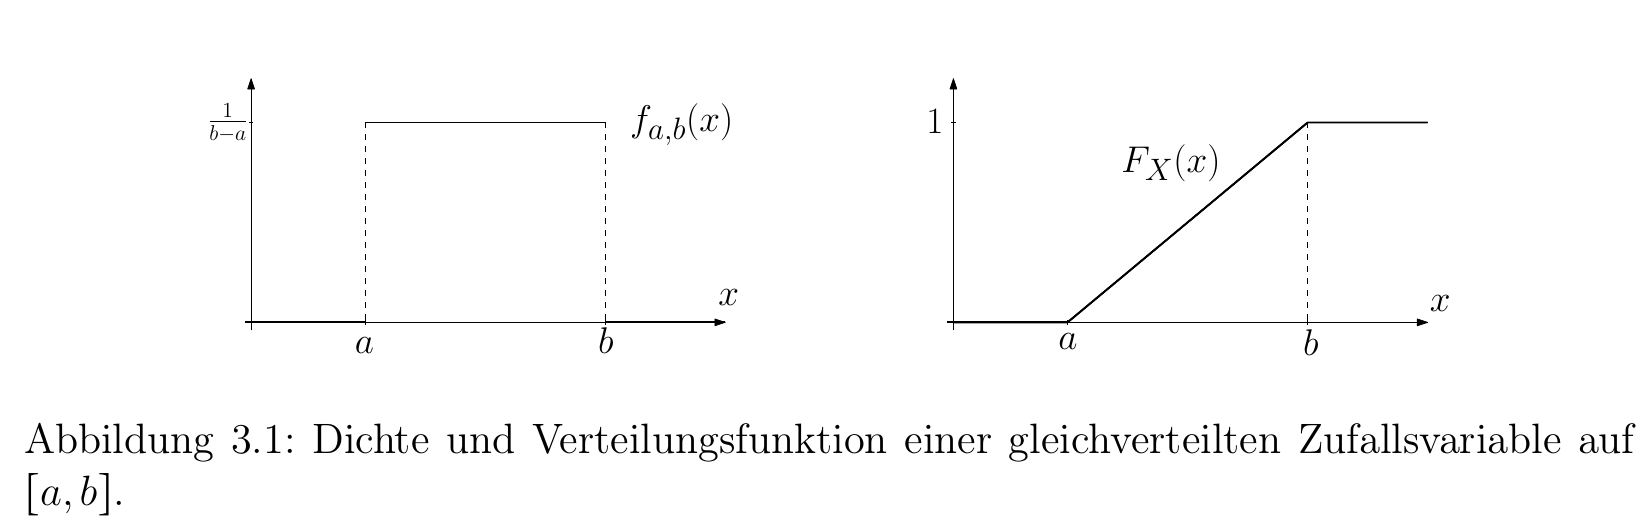
\includegraphics[scale=0.1]{Gleichverteilt.png}
\Bem[3.27A]
\begin{itemize}
    \item Die Wahrscheinlichkeit in einem Interval \( [c, c + \ell] \subset [a,b]\) zu fallen ist lediglich abhängig von dessen Länge \( \ell\) \[\mathbb{P}[X \in [c, c + \ell ]] = \frac{\ell}{b-a}\]
    \item Die Verteilungsfunktion X ist gegeben durch \[ F_X(x) = \begin{cases}
        0 & x < a \\
        \frac{x-a}{b-a} & a \leq x \leq b \\
        1 & x > b
    \end{cases}\]
\end{itemize}
\Def[3.28 Exponentialverteilung mit \(\lambda > 0\) ] \newline
Eine stetige Zufallsvariable T heisst exponentialverteilt mit Parameter \( \lambda > 0\) falls ihre Dichte gegeben ist durch
\[ f_\lambda(x) = \begin{cases}
    \lambda \exp ^{-\lambda x } & x \geq 0 \\
    0 & x < 0
\end{cases}\]
\Bem[3.28A]
Die Grafik zeigt die Dichte und Verteilungsfunktion einer exponentialverteilten Zufallsvariable mit Parameter \( \lambda\)
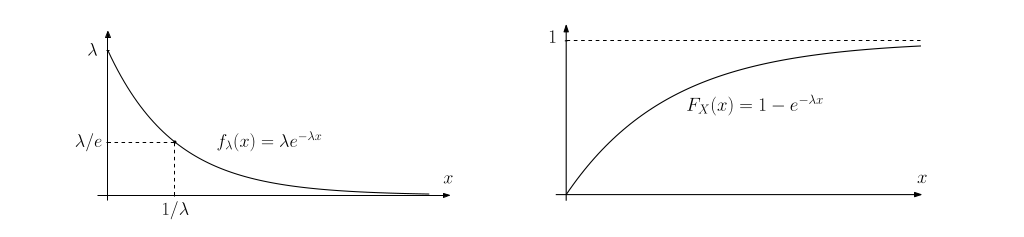
\includegraphics[scale=0.2]{exp_Dichte_Verteilung.png} \\ 
T modelliert häufig die Lebensdauer oder Wartezeit eines allgemeinen Ergebnisses. \\
Eigenschaften: \begin{itemize}
    \item Die Wahrscheinlichkeit des Wartens ist exponentiell klein: \[ \forall t \geq 0 \ \mathbb{P}[T > t] = \exp^{-\lambda t }\]
    \item T besitzt die Eigenschaft der Gedächnislosigkeit \[ \forall t,s > 0 \ \mathbb{P}[T > t + s | T > t] = [T > s]\]
\end{itemize}

\Def[3.29] \newline
Eine stetige Zufallsvariable X heisst normal verteilt mit Parametern m und \( \sigma^2 > 0\) falls ihre Dichte gegeben ist durch \[ f_{m,\sigma}(x) = \frac{1}{\sqrt{2 \pi \sigma^2}}\exp^{-\frac{(x-m)^2}{2 \sigma^2}}\]
Wir schreiben \( X \sim \mathcal{N}(m, \sigma^2)\) \newline
\Bem[3.29A] \newline
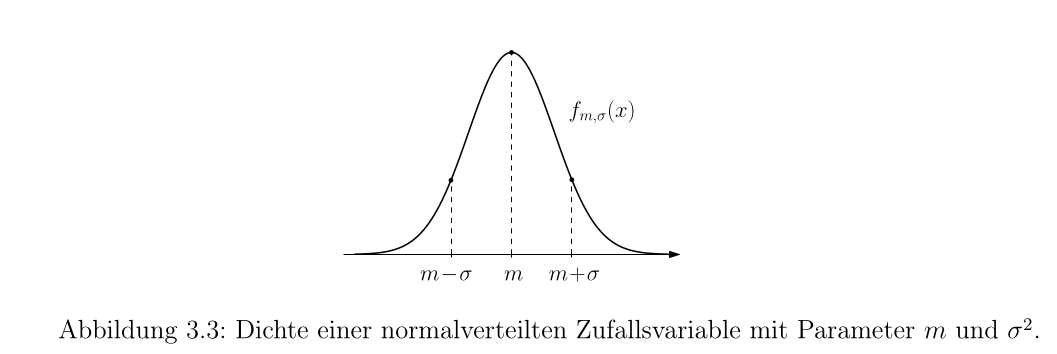
\includegraphics[scale=0.175]{Dichte_Normalverteilung.png} \\
Zum Beispiel bei einer physikalischen Messung kann der parameter \( \sigma\) die Schwankung von X darstellen und generell zeigt ein kleines \(\sigma\) eine genaue Messung an und ein grosses \(\sigma\) eine ungenaue.
Eigenschaften : \begin{itemize}
    \item Seien \(X_1, \dots X_n\) unabhängige normalverteilte Zufallsvariablen mit Parametern \((m_1, \sigma_1^2), \dots , (m_n, \sigma_n^2)\) dann ist \[ Z = m_0 + \lambda_1 X_1 + \dots + \lambda_n X_n \] eine normalverteilte Zufallsvariable mit Parametern \(m = m_0 + \lambda_1 m_1 + \dots + \lambda_n m_n\) und \(\sigma^2 = \lambda_1^2 \sigma_1^2 + \dots + \lambda_n^2 \sigma_n^2\)
    \item Wir sprechen im Fall von  \( X \sim \mathcal{N}(0,1)\), gerade von einer standardnormalverteilten Zufallsvariable. Man merke sich dann folgende Beziehung \[ Z = m + \lambda \cdot X\], wobei X eine normalverteilte Zufallsvariable mit Parametern m und \(\sigma^2\) ist.
    \item Falls X normalverteilt mit Parametern m und \( \sigma^2 \) ist, dann liegt die "meiste " Wahrscheinlichkeitsmasse der Z.V im Intervall \( [m - 3\sigma, m + 3\sigma ]\). Es gilt gerade \[ \mathbb{P}[\abs{X - m} \geq 3 \sigma ] \leq 0.0027\]
\end{itemize}


\end{multicols*}
\end{document}